\section{Serendipity in a computational context} \label{sec:computational-serendipity}

The 13 criteria from Section \ref{sec:literature-review}
specify the conditions and preconditions that are conducive to
serendipitous discovery.  Here, we revisit each of these criteria and
briefly summarise how they can be thought about from a computational
point of view.
% What is the goal of the computation (input and output)
% Why is it appropriate (formal spec e.g. considering externalities)
% what is the logic of the strategy by which it can be carried out.

\textbf{[We will have to make good on our promise to ``reinterpret van
    Andel's `patterns of serendipity' in computational settings'' or
    else drop it from the introduction.]}

% \newpage
\subsubsection*{Key condition for serendipity}

\begin{itemize}
\item \textbf{Focus shift}: A focus shift is linked to re-evaluation
  of data, processes, or products.  It may precipitate changes in the
  entire framework of evaluation or its effects may be more contained.
  Such reevaluation could be modelled using a multi-agent
  architecture, in which each agent has a goal and evaluates generated
  products relative this goal, but in which agents also share their
  products with other, who then evaluate them against their own
  metrics.
\end{itemize}

\subsubsection*{Components of serendipity}

\begin{itemize}
\item \textbf{Prepared mind}: This comprises the background knowledge,
  unsolved problems, current goal, programming, and operating
  environment of a computational system.
%%
\item \textbf{Serendipity trigger}: The generation or observation of a
  potentially novel example, concept, or conjecture, etc., which
  precedes a discovery in a computational system.\footnote{Triggers
    are often examples without an explanation, rather than
    wholly-formed concepts.}  The trigger is outside of the direct
  control of the system components responsible for evaluations.
%%
\item \textbf{Bridge}: Reasoning and/or programmatic interaction
  brings about a focus shift at an opportune juncture, building on
  prior preparation and on the serendipity trigger.  The bridge may be
  constructed on the basis of logical methods, analogies, conceptual
  blending, evolutionary search, automated theory formation and may
  draw on interactions with other systems.
%%
\item \textbf{Result}: The discovery itself may be a new product,
  artefact, process, hypothesis, use for an object, etc., generated by
  computational means, which may influence the future operations of
  the system.
\end{itemize}

\subsubsection*{Dimensions of serendipity}

\begin{itemize}
\item \textbf{Chance}: Controlled randomness in AI systems is
  well-established, e.g. in Genetic Algorithms and search.  Chance
  also applies in connection with an under-determined outside world
  (see below).
%%
\item \textbf{Curiosity}: The system needs to expend discretionary
  computational effort on the serendipity trigger.  This may be
  accompanied by system features that an observer would describe as
  playfulness, inventiveness, and the drive to experiment or
  understand.
%%
\item \textbf{Sagacity}: Sagacity be modelled by employing reasoning
  over multiple application domains simultaneously; or, again, with a
  social analogue in cases where the system does not know, but ``knows
  who to ask.''
%%
\item \textbf{Value}: The result should be interesting or useful, as
  judged by the system, the programmer, the user, or another party
  (potentially another system).
\end{itemize}

\subsubsection*{Environmental factors}

\begin{itemize}
\item \textbf{Dynamic world}: Connections with other systems, data
  sources, or user input, e.g., via the web, which is highly dynamic --
  or in the context of a larger simulation.
%%
\item \textbf{Multiple contexts}: Reasoning which operates across
  domains, such as analogical reasoning, or that considers multiple
  perspectives, as in systems with social awareness.
%%
\item \textbf{Multiple tasks}: Multiple goals or targets that compete
  for resources.  The system may be implemented using a multithreaded,
  parallel processing design.
%%
\item \textbf{Multiple influences}: This may again be modelled as a
  multi-agent systems, as or multiple interacting systems, each with
  different knowledge and goals.  The source of unexpectedness may be
  arise on various levels, and a system may bring this to bear using
  techniques of reflection.
\end{itemize}

% \subsection{Proposed experiment: A Writers Workshop for Systems} \label{sec:writers-workshop}

Richard Gabriel \cite{gabriel2002writer} describes the practise of
Writers Workshops that has been put to use for over a decade within
the Pattern Languages of Programming (PLoP) community.  The basic
style of collaboration originated much earlier with groups of literary
authors who engage in peer-group critique.  Some literary workshops
are open as to genre, and happy to accommodate beginners, like the
Minneapolis Writers
Workshop\footnote{\url{http://mnwriters.org/how-the-game-works/}};
others are focused on professionals working within a specific genre,
like the Milford Writers
Workshop\footnote{\url{http://www.milfordsf.co.uk/about.htm}}.  The
practices that Gabriel describes are fairly typical.  Authors come
with work ready to present, and read a short sample, which is then
discussed and constructively critiqued by attendees.  Presenting
authors are not permitted to rebut these comments.  The commentators
generally summarise the work and say what they have gotten out of it,
discuss what worked well in the piece, and talk about how it could be
improved.  The author listens and may take notes; at the end, he or
she can then ask questions for clarification.  Generally, non-authors
are either not permitted to attend, or are asked to stay silent
through the workshop, and perhaps sit separately from the
participating authors/reviewers.  There are similarities between the
Writers Workshops and classical practices of group composition
\cite{jin1975art} and dialectic \cite{dialectique}, and the workshop
may be considered an artistic or creative space in its own right.

In PLoP workshops, authors present design patterns and pattern
languages, or papers about patterns, rather than more traditional
literary forms like poems, stories, or chapters from novels.  Papers
must be workshopped at a PLoP or EuroPLoP conference in order to be
considered for the \emph{Transactions on Pattern Languages of
  Programming} journal.  A discussion of writers workshops
in the language of design patterns is presented by
Coplien and Woolf \cite{coplien1997pattern}.  Their patterns include:
\begin{center}
{\small
\begin{tabular}{l@{\hspace{.2cm}}l@{\hspace{.2cm}}l}
\emph{Open Review} & \emph{Safe Setting} & \emph{Workshop Comprises Authors} \\
\emph{Authors are Experts} & \emph{Community of Trust} & \emph{Moderator Guides the Workshop} \\
\emph{Thank the Author} & \emph{Selective Changes} & \emph{Clearing the Palate} \\
\end{tabular}
}
\end{center}

We propose that a similar pattern-based approach should be deployed
within the Computational Creativity community to design a workshop in
which the participants are computer systems instead of human authors.
The annual International Conference on Computational Creativity
(ICCC), now entering its sixth year, could be a suitable venue.
Rather than the system's creator presenting the system in a
traditional slideshow and discussion, or a system ``Show and Tell,''
the systems would be brought to the workshop and would present their
own work to an audience of other systems, in a Writers Workshop
format.  This might be accompanied by a short paper for the conference
proceedings written by the system's designer describing the system's
current capabilities and goals.  Subsequent publications might include
traces of interactions in the Workshop, commentary from the system on
other systems, and offline reflections on what the system might change
about its own work based on the feedback it receives.  As in the PLoP
community, it could become standard to incorporate this sort of workshop
into the process of peer reviewing journal articles for the new \emph{Journal of
  Computational Creativity}\footnote{\url{http://www.journalofcomputationalcreativity.cc}}.

\begin{table}[p]
\begin{tabular}{lp{.7\textwidth}}
{\bf\emph{Successful error}} & \\
\emph{Van Andel's example}: & Post-it\texttrademark\ notes \\[.2cm]
{\tt presentation}& Systems should be prepared to share interesting ideas even if they don't know directly how they will be useful.  \\
{\tt listening}   & Systems should listen with interest, too. \\
{\tt feedback}    & Even interesting ideas may not be ``marketable.''\\
{\tt questions}   & How is your suggestion useful? \\
{\tt reflections} & New combinations of ideas take a long time to realise, and many different ideas may need to be combined in order to come up with something useful.\\
\end{tabular}
\bigskip

\begin{tabular}{lp{.7\textwidth}}
{\bf\emph{Side effect}} & \\
\emph{Van Andel's example}: & Nicotinamide used to treat side-effects of radiation therapy proves efficacious against tuberculosis. \\[.2cm]
{\tt presentation}& Systems should use their presentation as an experiment. \\
{\tt listening}   & Listeners should allow themselves to be affected by what they are hearing. \\
{\tt feedback}    & Feedback should convey the nature of the effect.\\
{\tt questions}   & The presenter may need to ask follow-up questions to gain insight. \\
{\tt reflections} & Form a new hypothesis before seeking a new audience. \\
\end{tabular}
\bigskip

\begin{tabular}{lp{.7\textwidth}}
{\bf\emph{Wrong hypothesis}} & \\
\emph{Van Andel's example}: & Lithium, used in a control study, had an unexpected calming effect. \\[.2cm]
{\tt presentation}& How is this presentation interpretable as a (``natural'') control study? \\
{\tt listening}   & Listeners are ``guinea pigs''.\\
{\tt feedback}    & Discuss side-effects that do not necessarily correspond to the author's perceived intent. \\
{\tt questions}   & Zero in on the most interesting part of the conversation.\\
{\tt reflections} & Revise hypotheses to correspond to the most surprising feedback. \\
\end{tabular}
\bigskip

\begin{tabular}{lp{.7\textwidth}}
{\bf\emph{Outsider}} & \\
\emph{Van Andel's example}: & A mother suggests a new hypothesis to a doctor. \\[.2cm]
{\tt presentation}& The presenter is here to learn from the audience. \\
{\tt listening}   & The audience is here to give help, but also to get help.\\
{\tt feedback}    & Feedback will inevitably draw on previous experiences and ideas.\\
{\tt questions}   & What is the basis for that remark?\\
{\tt reflections} & How can I implement the suggestions?\\
\end{tabular}
\vspace{.2cm}
\caption{Reinterpreting patterns of serendipity for use in a computational workshop\label{tab:reinterpret}}
\end{table}

\begin{figure}[t]
\begin{center}
\resizebox{.93\textwidth}{!}{
\StickyNote[2.5cm]{myyellow}{{\LARGE {Interesting idea}} \\[4ex] {Surprise birthday party}}[3.8cm] \StickyNote[2.5cm]{mygreen}{{\Large I heard you say:} \\[4ex] {``surprise''} }[3.8cm]
\StickyNote[2.5cm]{pink}{{\Large Feedback:} \\[4ex] {I don't like surprises}}[3.8cm]
}
\resizebox{.61\textwidth}{!}{
\StickyNote[2.5cm]{myorange}{{\LARGE {Question}} \\[4ex] {Not even a little bit?\ldots}}[3.8cm]
\quad \raisebox{-.2cm}{\StickyNote[2.5cm]{myblue}{{\LARGE Note to self:} \\[4ex] {(Try smaller surprises \\ next time.)}}[3.8cm]}
}
\end{center}
\caption{A paper prototype for applying the \emph{Successful Error} pattern\label{fig:paper-prototype}}
\end{figure}

In order to facilitate this sort of interaction, it would be necessary
for systems to implement a basic protocol related to
%%
\[
\text{
{\tt presentation}, {\tt listening}, {\tt
  feedback}, {\tt questions}, and {\tt
  reflections}.}
\]
%%
This protocol could be thought of as a light-weight template for
creating design patterns that guide system-level participation in the
context specified by Coplien and Woolf's pattern language for writers
workshops.  Table \ref{tab:reinterpret} uses this framework to recast
the four ``perfectly'' serendipitous patterns from van Andel --
\emph{Successful error}, \emph{Side effect}, \emph{Wrong hypothesis},
and \emph{Outsider} -- in a form that may make them useful to
developers preparing to enter their systems into the Workshop.
%
Further guidelines for structuring and participating in traditional
writers workshops are presented by Linda Elkin in
\cite[pp. 201-203]{gabriel2002writer}.  It is not at all clear that
the same ground rules should apply to computer systems.  For example,
one of Elkin's rules is that ``Quips, jokes, or sarcastic comments,
even if kindly meant, are inappropriate.''  Rather than forbidding
humour, it may be better for individual comments to be rated as
helpful or non-helpful.  Again, since serendipitous discovery is an
overarching goal, in the first instance, usefulness and interest might
be judged in terms of the criteria described in Section
\ref{sec:evaluation-criteria}.

We would need a neutral environment that is not hard to develop for:
the {\sf FloWr} system described in Section \ref{sec:foundations}
offers one such possibility.  With this system, the basic operating
logic of the Workshop could be spelled out as a flowchart, and
contributing systems could use flowcharts as the basic medium for
sharing their presentations, feedback, and questions.  Developing
around a process language of this sort partially obviates the need for
participating systems to have strong natural language processing
capabilities.  
%
Post-it\texttrademark\ notes, which have provided us with a useful
example of serendipitous discovery, also provide indicative strategies
from the world of paper prototyping (Figure \ref{fig:paper-prototype}).

Gordon Pask's conversation theory, reviewed in
\cite{conversation-theory-review,boyd2004conversation}, goes
considerably beyond what we have presented here as a simple process
language, although there are structural parallels.  In a basic
Pask-style learning conversation: (0) Conversational participants are
carrying out some actions and observations; (1) naming and recording
what action is being done; (2) asking and explaining why it works the
way it does; (3) carrying out higher-order methodological discussion;
and (4) trying to figure out why unexpected results occured \cite[p. 190]{boyd2004conversation}.

Naturally, variations to the underlying system, protocol, and the
schedule of events should be considered depending on the needs and
interests of participants, and several variants can be tried.  On a
pragmatic basis, if the Workshop proved quite useful to participants,
it could be revised to run monthly, weekly, or
continuously.\footnote{For a comparison case in computer Go, see
  \url{http://cgos.computergo.org/}.}


\subsection{Some completely realistic examples}

\textbf{[Here we should put examples of real historical systems that
    were designed with serendipity in mind, or that can be interpreted
    that way.  We could also include some completely \emph{formal}
    system (like ``Markov Chain Monte Carlo'') and show how it
    \emph{might} operate in a serendipitous fashion, as well as what
    limitations it runs into in the process.]}

\subsection{A Writers Workshop for Systems} \label{sec:ww}

%% \textbf{[It would be good to go back over our other paper and make
%%     sure we make good on the idea in the Related Work section of the
%%     current paper that ``This earlier paper remains broadly
%%     indicative, however, and the ideas it describes can see
%%     considerable benefit from the more formal thinking we develop in
%%     the current work.''}

%% \textbf{In particular: at least one of the reviewers found the Writers
%% Workshop ``technologically unrealistic'' or similar, so let's try to
%% make sure we're not overpromising.  I think the other paper makes it
%% all fairly realistic.]}

%% In \cite{poetry-workshop}, we investigate the feasibility of using
%% designs of this sort in multi-agent systems that learn by sharing and
%% discussing partial understandings.  This earlier paper remains broadly
%% indicative, however, and the ideas it describes can see considerable
%% benefit from the more formal thinking we develop in the current work.

% \citeA{poetry-workshop} describes a Writers Workshop for poetry
%systems. 

Following \citeA{gabriel2002writer}
% we described a template for a pattern
% language for interactions in a computational poetry workshop, closely
we define a \emph{Workshop} to be an activity for two or more agents
consisting of the following steps:
%itemize?
{\tt presentation}, {\tt listening}, {\tt feedback}, {\tt questions},
and {\tt reflections}.  In general, the first and most important
feature of {\tt feedback} is for the listener to say what they heard;
in other words, what they find in the presented work.  In some
settings this is augmented with {\tt suggestions}.  After any {\tt
  questions} from the author, the commentators may make {\tt replies}
to offer clarification.  This is how these steps map into the diagram
we introduced in Section \ref{sec:background}:

\begin{center}
\begingroup
\tikzset{
block/.style = {draw, fill=white, rectangle, minimum height=3em, minimum width=3em},
tmp/.style  = {coordinate}, 
sum/.style= {draw, fill=white, circle, node distance=1cm},
input/.style = {coordinate},
output/.style= {coordinate},
pinstyle/.style = {pin edge={to-,thin,black}}
}

\begin{tikzpicture}[auto, node distance=2cm,>=latex']
    \node [sum] (sum1) {};
    \node [input, name=pinput, above left=.9cm and .9cm of sum1] (pinput) {};
    \node [input, name=tinput, left=2.2cm of sum1] (tinput) {};
    \node [input, name=minput, below left of=sum1] (minput) {};
    \node [input, name=minput, right of=sum1] (moutput) {};
    \draw [->] (tinput) -- node{\vphantom{{\footnotesize g}}{\footnotesize \emph{presentation}~~}} (sum1);
    \draw [->] (pinput) -- node{{\footnotesize listening}} (sum1);
    \draw [->] (sum1) -- node{\vphantom{{\footnotesize g}}{\footnotesize feedback}}  (moutput);
\end{tikzpicture}
\hspace{1cm}
\begin{tikzpicture}[auto, node distance=2cm,>=latex']
    \node [sum] (sum1) {};
    \node [input, name=pinput, above left=.9cm and .9cm of sum1] (pinput) {};
    \node [input, name=tinput, left of=sum1] (tinput) {};
    \node [input, name=minput, below left of=sum1] (minput) {};
    \node [sum, right=1.5cm of sum1] (sum2) {};
    \node [input, name=minput, right of=sum2] (moutput) {};
    \draw [->] (tinput) -- node{\vphantom{{\footnotesize g}}{\footnotesize feedback~~}} (sum1);
    \draw [->] (pinput) -- node{{\footnotesize \emph{questions}}} (sum1);
    \draw [->] (sum1) -- node{\vphantom{{\footnotesize g}}{\footnotesize answers}} (sum2);
    \draw [->] (sum2) -- node{{\footnotesize \emph{reflections}}}  (moutput);
\end{tikzpicture}
\endgroup
\end{center}

%% {\centering
%% 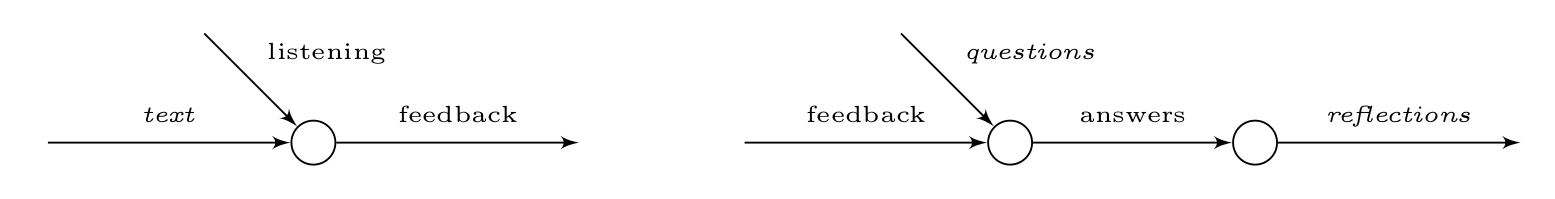
\includegraphics[width=.9\textwidth]{ww-serendipity-diagram}
%% \par}

Italicised elements (\emph{presentation}, \emph{questions}, and
\emph{reflections}) are the responsibilities of the presenting author,
and the upright elements (listening, feedback, and
answers) are the responsibilities of the attendant critics.
%
The system as a whole can be further decomposed into generative
components as follows:

\bigskip

\begin{tikzpicture}[
single/.style={draw, anchor=text, rectangle},
]
\node (discovery) {\textbf{\emph{Discovery:}}};
% poet generates poem
\node[single, right=8mm of discovery.east,text width=1.5cm] (poet) {\emph{poetry generator}};
\node[single, right=4mm of poet.east] (poem) {P};
\draw [-latex] (poet.east) -- (poem.west);
% critic listens to poem and offers feedback
\node[single, right=4mm of poem.east,text width=1.5cm] (critic) {comment generator};
\draw [-latex] (poem.east) -- (critic.west);
\node[single, right=4mm of critic.east] (feedback) {F};
\draw [-latex] (critic.east) -- (feedback.west);

%%% Next phase
\node[below=1cm of discovery] (invention) {\textbf{\emph{Invention:}}};
% poet integrates feedback
\node[single, right=8mm of invention.east] (feedbackcont) {F};
\node[single, right=8mm of feedbackcont.east,text width=1.7cm] (integrator) {\emph{feedback integrator}};
\draw [-latex] (feedbackcont.east) -- (integrator.west);

\node[single, below=8mm of integrator.south,text width=1.5cm] (explainer) {feedback explainer};

\node[single, below right=2mm and 2mm of integrator] (question) {Q};
\node[single, below left=2mm and 2mm of integrator] (answer) {A};

\draw[-latex] ([yshift=-1.5mm]integrator.east) to [out=0,in=90] (question.north) ;
\draw[-latex] (question.south) to [out=270,in=0] (explainer.east) ;
\draw[-latex] (explainer.west) to [out=180,in=270] (answer.south) ;
\draw[-latex] (answer.north) to [out=90,in=180] ([yshift=-1.5mm]integrator.west) ;

\node[single, right=8mm of integrator.east] (problem) {X};

\draw [-latex] (integrator.east) -- (problem.west);

% poet reflects on feedback and updates codebase

\node[single, right=4mm of problem.east,text width=1.5cm] (pgrammer) {\emph{code}\\ \emph{generator}};

\draw [-latex] (problem.east) -- (pgrammer.west);

\node[single, right=4mm of pgrammer.east,text width=.3cm] (etc) {...};

\draw [-latex] (pgrammer.east) -- (etc.west);
\end{tikzpicture}


\noindent (We focus here on the case of a poetry workshop; similar
ideas would apply for prose and other arts.)

\paragraph{Writers Workshop: Prepared mind.}
Participating systems need to be able to follow the protocol.  This
means that participating systems will need components like those
listed above. The {\tt listening} and {\tt questions} components of
the protocol correspond to $p$ and $p^{\prime}$ our model of
serendipity.  The corresponding ``comment generator'' and ``feedback
integrator'' modules in the architecture represent the primary points
of interface to the outside world.  In principle these modules need to
be prepared to deal (more or less thoughtfully) with \emph{any} text,
and in turn, with \emph{any} comment on that text.  Certain limits may
be agreed in advance; e.g.~as to genre or length in the case of texts,
and what constitutes an acceptable comment.  The ``feedback
explainer'' is closely connected with the ``comment generator'' and in
an implementation of this model they would presumably share a
codebase.  The loop for learning by asking questions as they arise is
reminiscent of the operating strategy of {\sf SHRDLU}
\cite{winograd1972understanding}.

\paragraph{Writers Workshop: Serendipity triggers.}

Although the poem is under the control of the initial generative
subsystem, it is \emph{not} under control of the listening subsystem.
The listening subsystem expects some poem, but it does not know what
poem to expect.  In this sense, the poem constitutes a serendipity
trigger $T$, not only for the listening subsystem, but for the
Workshop system as a whole.

To expand this point, note that there may be several listeners, each
sharing their own feedback and listening to the feedback presented by
others (which, again, is outside of their direct control).  This
creates further potential for serendipity, since each listener can
learn what others see in the poem.  More formally, in this case
$T^\star$ may seen as an evolving vector with shared state, but viewed
and handled from different perspectives.  With multiple agents
involved in the discussion, the ``comment generator'' module would
expand to contain its own feedback loops.

\paragraph{Writers Workshop: Bridge.}

Feedback on portions of the poem may lead the system to identify new
problems, indeed, new \emph{types} of problems that it hadn't
considered before.  The most immediately feasible case is one in which
the critic is a programmer who can directly program new concepts into
the computer \cite<cf.>{winograd1972understanding}.  However, it would
be hard to call that ``serendipity.''

We can also ask whether agents can build new concepts \emph{without}
outside intervention, starting with some basic concepts and abilities
related to poetry (e.g.~definitions of words, valence of sentiments,
metre, repetition, density, etc.) and code (e.g.~the data, functions,
and macros in which the poetic concepts and workshop protocols are
embodied).  Previous experiments with concept invention have been
fraught with questions about autonomy
\cite{ritchie1984case,lenat1984and}.  One cognitively inspired
hypothesis is that the formation of new concepts is closely related to
formation of sensory experiences \cite{milan2013kiki}.  If the
workshop participants have the capacity to identify the distinctive
features of a given poem, then training via a machine learning or
genetic algorithm approach could be used assemble a battery of
existing low-level tools that can approximate the effect.  Relatedly,
a compression process could seek to produce a given complex poetic
effect with a maximally-succinct algorithm.

The key point is that feedback on the poem -- simply describing what's
in the poem from several different points of view -- can be used to
define new problems for the system to solve.  This is not simply a
matter of decomposing the poem into pieces, but also of reconstructing
the way in which the pieces work together.  This is one of the
functions of the {\tt questions} step corresponding to $p^{\prime}$ in
our formalism: they offer the poet the opportunity to enquire about
how different pieces of feedback fit together, and learn more about
where they come from.  Although computers are currently nowhere close,
the reconstructive process may steadily approach the ideal case --
familiar to humans -- of relating to the sentiment expressed by the
poem as a whole \cite[p. 209]{bergson1983creative}.

%% Several of us are involved with a contemporary project
%% \cite{coinvent14} to develop a formal theory of concept invention,
%% focusing on \emph{concept blending}.  The additive or subtractive
%% blending of existing poetry profiles may be another way to create new
%% concepts.


%% should be possible Modifer Grammar
%% Counting Breathing Position Distribution Phonics Rhythm Repetition
%% Thematic Narrative Entropy

\paragraph{Writers Workshop: Result.} 

The final step is to take the problem or problems that were
identified, and write new code to solve them.  Several strategies for
generating a result $R$, in the form of new code, were described
above.  Now the system evaluates the new code to see whether it holds
promise.  In order to do this, it must have a way to carry out an
evaluation and judge whether $|R|>0$.  In the most straightforward
case, it would simply make changes to the draft poem that seem to
improve it in some way.  For example, the might remove material that
elicited a negative response from a critic.  It may update its modules
related to poetry generation.  Notably, it may also update its own
feedback modules, after reflecting on questions like: ``How was the
critic able to detect that feature in my poem?''
